\documentclass[10pt]{article}
\usepackage[utf8]{inputenc}
\usepackage[T1]{fontenc}
\usepackage[margin=0.95in]{geometry}
\usepackage{amsmath,amssymb,amsthm}
\usepackage{booktabs}
\usepackage{array}
\usepackage{url}
\usepackage{microtype}
\usepackage{graphicx}
\usepackage{caption}
\usepackage{xcolor}
\usepackage[hidelinks]{hyperref}
\makeatletter\g@addto@macro{\UrlBreaks}{\do\_\do\.\do\/}\makeatother
\emergencystretch=3em
\tolerance=2000
% generated by make_all.py from code/*.json; do not edit
\newcommand{\BEBcc}{\ensuremath{-1.4442308}}
\newcommand{\BGapFcc}{\ensuremath{8.969\times10^{-5}}}
\newcommand{\BGapHcp}{\ensuremath{1.469\times10^{-4}}}
\newcommand{\BRelGapFcc}{\ensuremath{6.21\times10^{-5}}}
\newcommand{\BSlackRadial}{\ensuremath{3.091\times10^{-3}}}
\newcommand{\BSlackAxial}{\ensuremath{1.058\times10^{-4}}}
\newcommand{\BSlackHier}{\ensuremath{8.751\times10^{-5}}}
\newcommand{\BSlackAzi}{\ensuremath{5.574\times10^{-5}}}
\newcommand{\BSlackAxHex}{\ensuremath{3.745\times10^{-5}}}
\newcommand{\BSlackAxSq}{\ensuremath{1.830\times10^{-5}}}
\newcommand{\BRatioRadial}{\ensuremath{34.5}}
\newcommand{\BRatioAxial}{\ensuremath{1.18}}
\newcommand{\BRatioHier}{\ensuremath{0.98}}
\newcommand{\BRatioAxialHcp}{\ensuremath{0.72}}
\newcommand{\BNSigmaHier}{\ensuremath{303}}
\newcommand{\BNSigmaAx}{\ensuremath{448}}
\newcommand{\BSeedAxA}{\ensuremath{1.0586\times10^{-4}}}
\newcommand{\BSeedAxB}{\ensuremath{1.0576\times10^{-4}}}
\newcommand{\BSeedHierA}{\ensuremath{8.7547\times10^{-5}}}
\newcommand{\BSeedHierB}{\ensuremath{8.7477\times10^{-5}}}
\newcommand{\BWSAx}{\ensuremath{1.3\times10^{-30}}}
\newcommand{\BWSRad}{\ensuremath{2.2\times10^{-30}}}
\newcommand{\BWSHier}{\ensuremath{1.3\times10^{-30}}}
\newcommand{\BLapFD}{\ensuremath{12.5656}}
\newcommand{\BLapExp}{\ensuremath{12.5664}}
\newcommand{\BGradDev}{\ensuremath{9.0\times10^{-9}}}
\newcommand{\BHexA}{\ensuremath{8.88\times10^{-6}}}
\newcommand{\BHexB}{\ensuremath{5.72\times10^{-4}}}
\newcommand{\BHexC}{\ensuremath{6.60\times10^{-3}}}
\newcommand{\BHexSixC}{\ensuremath{3.30\times10^{-3}}}
\newcommand{\BSqFourC}{\ensuremath{5.85\times10^{-3}}}
\newcommand{\BOffHex}{\ensuremath{6.9\times10^{-17}}}
\newcommand{\BOffSq}{\ensuremath{8.0\times10^{-17}}}
\newcommand{\BCFour}{\ensuremath{-2.77}}
\newcommand{\BCFourFcc}{\ensuremath{-1.55}}
\newcommand{\BCFourSc}{\ensuremath{7.60}}
\newcommand{\BCReg}{\ensuremath{-2.88847}}
\newcommand{\BTwoMad}{\ensuremath{-2.88846}}
\newcommand{\BDRadTwoD}{\ensuremath{1.85\times10^{-3}}}
\newcommand{\BDGapTwoD}{\ensuremath{0.03325}}
\newcommand{\BDRatioTwoD}{\ensuremath{0.056}}
\newcommand{\BTwoGap}{\ensuremath{1.7938\times10^{-4}}}
\newcommand{\BMNMargin}{\ensuremath{1.7938\times10^{-4}}}
\newcommand{\BNodesTwoD}{\ensuremath{7.89\times10^{6}}}
\newcommand{\BMarginRatio}{\ensuremath{129}}
\newcommand{\BRefine}{\ensuremath{11.4}}
\newcommand{\BNodesThreeD}{\ensuremath{3.2\times10^{13}}}
\newcommand{\BCoreYears}{\ensuremath{221}}
\newcommand{\BNodesFiveD}{\ensuremath{3.3\times10^{22}}}
\newcommand{\BEpsPerNode}{\ensuremath{2.1\times10^{-4}}}
\newcommand{\BNEulerCfg}{29}
\newcommand{\BNCfgAll}{32}
\newcommand{\BAlphaSpread}{\ensuremath{8.9\times10^{-16}}}
\newcommand{\BMadDev}{\ensuremath{2.8\times10^{-13}}}
\newcommand{\BMadDevSc}{\ensuremath{2.1\times10^{-9}}}
\newcommand{\BNegSpread}{\ensuremath{0.44}}
\newcommand{\BNNotTwelve}{3}
\newcommand{\BHcpArtifact}{\ensuremath{11.9375}}
\newcommand{\BTableConfigs}{%
bcc & 1 & 0 & 14.00 & 12.00 & 0.0785433\\
fcc & 1 & $8.97\times10^{-5}$ & 12.00 & 24.00 & 0.0787451\\
hcp & 2 & $1.47\times10^{-4}$ & 12.00 & 24.00 & 0.0787451\\
A15 (Weaire--Phelan) & 8 & $3.37\times10^{-3}$ & 13.50 & 12.00 & 0.0787354\\
C15 & 24 & $1.58\times10^{-2}$ & 13.33 & 12.00 & 0.0793381\\
sc & 1 & $2.56\times10^{-2}$ & 6.00 & 12.00 & 0.0833333\\
fcc, perturbed (rms amplitude 0.002, seed 1) & 64 & $1.10\times10^{-4}$ & 14.00 & 12.00 & 0.0787463\\
Poisson, $N=400$, seed 1 & 400 & -- & 15.50 & 12.00 & 0.1158316\\}

\newcommand{\tier}[1]{\textsf{[#1]}}
\newcommand{\cid}[1]{\texttt{B3-#1}}
\newcommand{\R}{\mathbb{R}}
\newcommand{\W}{\mathcal{W}}
\newcommand{\dd}{\mathrm{d}}
\newtheorem{lemma}{Lemma}
\newtheorem{proposition}{Proposition}
\theoremstyle{remark}
\newtheorem{remark}{Remark}

\title{Can the planar Sandier--Serfaty proof architecture reach three-dimensional bcc jellium?\\
A feasibility study with a negative outcome}
\author{Xavier Callens (SocrateAI Lab)}
\date{Preprint v1, 2026-10-26}
\hypersetup{pdftitle={Can the planar Sandier-Serfaty proof architecture reach three-dimensional bcc jellium? A feasibility study with a negative outcome},
  pdfauthor={Xavier Callens}}

\begin{document}
\maketitle
\begin{center}\small doi:10.5281/zenodo.23655002 \quad (not peer reviewed)\end{center}

\begin{center}\small Zenodo DOI to be assigned on release \quad (not peer reviewed)\end{center}

\noindent\textbf{AI-assistance disclosure.} This preprint, its Python code, its figures and its claim ledger were produced by AI agents
(Claude, Anthropic) under the author's direction. The author is responsible for the content. No human has checked the hand arguments
(Tier~C) or reviewed the numerics. One independent AI audit (a separate Claude agent instance that did not write the study or the paper; verdict
``accept with corrections'', corrections applied in this version; file \texttt{AUDIT.md}) has been done; \emph{no human audit has been done}. The producer of the study and the writer of
the paper are instances of the same AI pipeline, and the ``demonstration'' in Section~\ref{sec:obstruction} is a human-style argument written
by an agent, not machine-checked. The mathematics under study (the planar proof) was itself produced by an AI system (the openai/math
release) and is not peer reviewed.

\begin{abstract}
Sandier and Serfaty conjectured that the triangular lattice minimizes the renormalized Coulomb energy of a planar point set in a
uniform background. A preprint in the openai/math release (AI-generated, not peer reviewed) claims a proof by a reduction to square tori,
a glued trial potential with an \emph{exact calibration} at the triangular lattice, and a finite computer certificate; our independent
reproduction and audit of it is doi:10.5281/zenodo.23653827. The three-dimensional analogue, Wigner's conjecture that the bcc lattice
minimizes the jellium energy among \emph{all} point sets, is open; bcc is known to be optimal only among Bravais lattices (Muratov--Novaga,
arXiv:2610.29732). We ask whether the planar architecture can be transcribed to bcc. \textbf{Outcome: negative for the literal transcription (radial, axial and piece-intrinsic trial classes); only heuristically negative for richer classes.}
We give a step-by-step decomposition of the planar proof into 13 steps and classify each as dimension-agnostic, transferable, or genuinely
planar. The incidence count (a per-cell Euler identity, $\sum_F(6-n_F)=12$ for simple cells) is \emph{not} the obstruction. The obstruction is the
exact calibration: the planar Green function is a function of two variables in every sector because $\cos 6m\varphi=T_{6m}(d/t)$,
whereas the bcc Green function restricted to a face circle at fixed distance $t$ carries a $\cos6\psi$ mode on hexagonal faces and a
$\cos4\psi$ mode on square faces (Tier~X). By a projection argument (Tier~C, a hand argument evaluated in floating point, not a rigorous enclosure) every certified constant from a radial, axial or
hierarchical trial class whose data are invariant under the $60^\circ$ rotation of the hexagonal pyramids (the number of parameters is not a hypothesis) is at most $W_{\rm bcc}-\delta$ with $\delta\ge\BSlackHier$ (hierarchical) or
$\delta\ge\BSlackAxial$ (axial; $\BRatioAxial$ times the fcc--bcc gap $\BGapFcc$); these slack values are floating-point Monte Carlo results.
For richer ansatz classes whose data are not invariant under that rotation (in particular classes that carry neighbour data) the negative rests only on a counting heuristic (about 12 conditions for 3 multipliers,
against 3 for 3 in 2D; Tier~C) and is \emph{not} a theorem. We state a weaker, non-sharp residual target (a computer-assisted improvement of the
Lieb--Narnhofer constant $-1.4508$ towards $-1.44423$), a falsification test for it, and a certificate-size estimate under explicit assumptions
(about $\BNodesThreeD$ nodes, of the order of $10^2$ core-years, for a uniform mesh in the best case). We prove nothing about bcc.
\end{abstract}

\section{Scope and conventions}\label{sec:scope}
\textbf{Question.} Does the architecture of the planar proof (Section~\ref{sec:arch}) transfer to three dimensions, with the bcc lattice in the
role of the triangular lattice? This is a feasibility study. It proves no theorem about bcc and it does not claim that bcc is, or is not, the
minimizer; it claims a negative about one proof strategy, within the scope stated in Section~\ref{sec:scope-neg}.

\textbf{Tiers.} Every claim carries one of four tags, matching the Elenchus claim ledger shipped with the paper
(\texttt{ledger/}, identifiers \cid{L-nnnn}, \cid{C-nnnn}, \cid{X-nnnn}).
\tier{L} is a theorem-like statement quoted from a source and accepted by the Elenchus citation gate.
\tier{C} is a human-style argument (or a literature remark quoted verbatim but not gateable), not machine-checked.
\tier{X} is a floating-point result of our own code, with controls; it never supports a claim by itself.
\tier{A} (kernel-checked) is empty: nothing here is formalized.
\emph{Re-tiering note.} The internal feasibility note used ``A'' for elementary inequalities with a proof sketch. In the ledger, A means
kernel-checked and an argument is capped at C, so these inequalities are filed and tagged C here. Anything that depends on a floating-point
number is filed at X (tier closure); e.g.\ the statement ``the slack is at least $8.75\times10^{-5}$'' is X, while the lemma that turns a
slack into a ceiling is C.

\textbf{Setting.} Unit density, $1/r$ Coulomb interaction, per-particle units. For a periodic configuration with background, $h$ solves
$-\Delta h=4\pi(\sum_p\delta_p-1)$ and $W(h)=\frac1{8\pi}\int^{\rm ren}|\nabla h|^2$ is the renormalized energy (the jellium energy per particle, e.g.\ $\BEBcc$ for bcc). The status of the problem: Lieb--Narnhofer prove
$e_{\rm Jell}\ge-1.4508\,\rho^{1/3}$ and the conjectured value is $-1.44423\,\rho^{1/3}$ \tier{C}\,(\cid{C-0001},\cid{C-0002}); bcc is optimal among
Bravais lattices \tier{L}\,(\cid{L-0001}), and for the Yukawa interpolation among lattices \tier{L}\,(\cid{L-0003}); the non-periodic bcc problem is called ``a
substantially harder three-dimensional crystallization problem'' by Muratov and Novaga \tier{C}\,(\cid{C-0005}).

\section{The planar architecture, step by step}\label{sec:arch}
The planar proof in the openai/math preprint~\cite{oai} is, as audited in~\cite{audit}, a chain of steps; we take it as given
(our audit found no gap in its Sections~2--5; \tier{C}\,\cid{C-0019}). We did not re-read the manuscript ourselves for this paper; the table follows our feasibility
note and the earlier audit. The independent audit of this preprint did re-read the planar manuscript's \texttt{04-calibration.tex} (Lemmas \texttt{cal:stationarity}, \texttt{cal:energy-identity}, the trial potential \texttt{cal:trial-potential}) and found our description of G5--G9 accurate. Table~\ref{tab:steps} lists the steps G1--G13 and our classification for 3D.

\begin{table}[h]
\centering\small
\begin{tabular}{@{}p{0.04\linewidth}p{0.36\linewidth}p{0.54\linewidth}@{}}
\toprule
\# & Planar step & Three-dimensional status\\
\midrule
G1 & Reduction from the plane to square tori (Sandier--Serfaty 2012) & Needs a 3D analogue. Exists for the smeared energy (Rougerie--Serfaty Thm.~1, \tier{L} \cid{L-0004}); but for $d\ge3$ the cutoff energy may depend on the cutoff (their Remark~B.2, \tier{C} \cid{C-0004}), so the planar statement ``for every field'' has no verified 3D counterpart; the statement about the minimum transfers.\\
G2 & Existence of a torus minimizer, pair-energy form & Dimension-agnostic (same argument).\\
G3 & Separation via a screened potential, $r_*=1/\sqrt\pi$ & Dimension-agnostic: $R=(3/4\pi)^{1/3}\approx0.6204$, face distance $\ge0.3102$ (\tier{C} \cid{C-0016}).\\
G4 & Incidence count: at most $6n$ sectors times a constant $K<0$ & Transfers: a per-cell Euler identity gives the count weight, with $K\le0$ (Section~\ref{sec:euler}; \tier{C} \cid{C-0014}, \cid{C-0015}). \emph{Not the obstruction.}\\
G5 & Gluing of $H=B(r)+\sum_k(r/t)^kD_k(t)$ across sectors & Dimension-agnostic for the \emph{axial} ansatz: ray-wise $t(\omega)=d/(\hat n\!\cdot\!\omega)$ agrees on interfaces.\\
G6 & Dual identity $W=\sum J(S)+\tfrac12\!\int|\nabla(h-H)|^2$ & Dimension-agnostic (Lemma~\ref{lem:dual}).\\
G7 & Sector integral $\to$ primitive $g_d(x)$ in 2 variables & Needs a 3D analogue: a primitive $\Gamma_{d,s}(x)$ in 3 variables (\tier{C}, not carried out).\\
G8 & \textbf{Exact calibration: $H=h_{\rm opt}$, square term zero} ($\cos k\varphi=T_k(d/t)$) & \textbf{Genuinely planar: fails} (Section~\ref{sec:obstruction}).\\
G9 & Stationarity: 2 multipliers solve 2 equations at a single sector type & Genuinely planar by counting (Section~\ref{sec:count}; \tier{C} heuristic).\\
G10 & Hexagon optimality behind the scalar bounds (Fejes T\'oth/Gruber) & Genuinely planar: the cell-local 3D analogues are open (Gersho) or false (Kelvin) (Section~\ref{sec:cells}).\\
G11 & Tails and lattice sums & Routine: cubic harmonics replace $z^{6m}$; $c_4\ne0$ (\tier{X} \cid{X-0003}).\\
G12 & Finite certificate with a Hessian at the stationary point & Needs a 3D analogue; size in Section~\ref{sec:cert}; not binding.\\
G13 & Separation used only for the minimizer & Dimension-agnostic.\\
\bottomrule
\end{tabular}
\caption{The planar proof as 13 steps and their three-dimensional status.}\label{tab:steps}
\end{table}

The essential mechanism, which Section~\ref{sec:obstruction} makes precise, is this. After the dual identity (G6) the whole proof is a
\emph{lower bound by a trial potential}: one chooses $H$ in a small family, so that $F(H)$ splits into local terms $J(S)$ that a finite
certificate can bound below; the proof is sharp only if the trial $H$ equals the true Green function $h$ at the optimizer. That
exactness is G8, and the ``multipliers'' of G9 are what make the local inequalities tight at one configuration.

\section{The dual identity and the ceiling}\label{sec:dual}
\begin{lemma}[dual identity; \tier{C}, \cid{C-0010}]\label{lem:dual}
Let $H$ be a trial potential with the same $1/r$ singularities as $h$, and $u=h-H$. Then
$\int|\nabla h|^2=\int|\nabla u|^2+2\!\int\!\nabla h\!\cdot\!\nabla H-\int|\nabla H|^2$, and the equation for $h$ gives
$\int\nabla h\!\cdot\!\nabla H=4\pi\big(H_{\rm reg}(0)-\int H\big)$. Hence
\[
W(h)=F(H)+\frac1{8\pi}\int|\nabla(h-H)|^2,\qquad F(H)=\sum_{\rm cells}\Big[-\!\int H-\frac1{8\pi}\int^{\rm ren}|\nabla H|^2\Big],
\]
with the constant term of the singular expansion normalized to zero. So $F(H)\le W(h)$ for every admissible $H$, with equality iff $H=h$.
\end{lemma}
The renormalization at the sites is inherited from the planar proof and is not re-derived here; the quantity we use below is only the
\emph{square term} $\mathrm{sl}(H)=\frac1{8\pi}\int|\nabla(h-H)|^2\ge0$.

\begin{lemma}[ceiling; \tier{C}, \cid{C-0012}]\label{lem:ceiling}
Suppose a method certifies a constant $C$ with $F(H_{\rm conf})\ge CN$ for every configuration to which the method applies (in the planar architecture: separated configurations, G13), where $H_{\rm conf}$ ranges over a class $\mathcal K$ of trial
potentials. Applying this to the bcc torus, $C\le F(H_{\rm bcc})/N=W_{\rm bcc}-\mathrm{sl}(H_{\rm bcc})\le W_{\rm bcc}-\inf_{H\in\mathcal K}\mathrm{sl}(H)$.
\end{lemma}
This does not use that bcc is the minimizer: bcc is simply one admissible configuration. It is separated (nearest-neighbour distance $(\sqrt3/2)2^{1/3}\approx1.091>R\approx0.620$), so the lemma applies to it. Hence $\delta_{\mathcal K}=\inf_{\mathcal K}\mathrm{sl}$ is the
\emph{best possible deficit} of the method. In the plane, $\delta_{\mathcal K}=0$ at the triangular lattice (Section~\ref{sec:obstruction}), and the certified constant can equal $W_{\rm tri}$;
in 3D, any $\delta_{\mathcal K}>0$ means the method cannot return $W_{\rm bcc}$.

\section{The obstruction: exact calibration fails in 3D}\label{sec:obstruction}
\subsection{A lower bound for the square term}
\begin{lemma}[slack lemma; \tier{C}, \cid{C-0011}]\label{lem:slack}
(i) If $\nabla H(x)$ lies in a subspace $N(x)$ for every $H\in\mathcal K$, then $|\nabla(h-H)|^2\ge|P_{N(x)^\perp}\nabla h|^2$ pointwise. For $H=H(r)$ this is the tangential gradient
$|\nabla_{\tan}h|^2$; for an axial $H(r,\theta)$ about a face normal $\hat n$ it is $(\hat e_\psi\!\cdot\!\nabla h)^2$, with $\psi$ the azimuth about $\hat n$.
(ii) If $R$ is an isometry of a piece fixing the apex and preserving the Dirichlet form and the singular part, and $H=H\circ R$, then $(1-R)(h-H)=(1-R)h$, and since $\|(1-R)/2\|\le1$,
$\|\nabla(h-H)\|\ge\tfrac12\|\nabla(h-h\circ R)\|$.
(iii) Squared Dirichlet distances add over pieces with disjoint interiors, and the maximum of two valid lower bounds is valid.
\end{lemma}
\emph{Proof.} (i) is Pythagoras for the decomposition of $\nabla h$ along $N(x)$ and $N(x)^\perp$. (ii) $H=H\circ R$ gives $(1-R)H=0$; $R$ is unitary in the Dirichlet inner product, so $\|(1-R)u\|\le2\|u\|$. (iii) is additivity of the integral. \qed

\textbf{Trial classes.} All three are defined on the Voronoi cell of the bcc lattice, a truncated octahedron with 8 regular hexagonal and 6 square faces; each face $F$ at distance $d$ from the site carries the pyramid with apex at the site.
\begin{itemize}
\item \emph{Radial}: $H=H(r)$ in each cell (the Lieb--Narnhofer-like class). Bound: (i) with the tangential gradient.
\item \emph{Axial}: $H=H(r,\theta)$ on each pyramid, rotationally symmetric about the face normal; this is the literal 3D transcription of the planar sector ansatz $H=B(r)+\sum_k(r/t)^kD_k(t)$ (since on the ray $t=d/\cos\theta$). On a hexagonal pyramid an axial $H$ is invariant under the $60^\circ$ rotation $R$ about $\hat n$, so (ii) applies there. Bound: $\max\{\text{(ii) on hexagonal pyramids},\text{(i) azimuthal on hexagonal pyramids}\}+\text{(i) azimuthal on square pyramids}$.
\item \emph{Hierarchical, piece-intrinsic}: $H$ built from in-face sectors whose data depend only on the sector itself (the face distance $d$ and in-face parameters). The six in-face sectors of a regular hexagonal face are congruent, so the same data force invariance under $R$. Bound: (ii) on hexagonal pyramids only; square pyramids are not used, so a larger bound is expected.
\end{itemize}
The classes are nested, radial $\subset$ axial $\subset$ hierarchical on the hexagonal pyramids, so a larger class has a smaller or equal slack.
The number of parameters is not a hypothesis: what the bound uses is invariance under $R$ (or the axial or radial structure), so a piece-intrinsic class with ten parameters is covered, while a two-parameter class that reads neighbour data is not. A class whose data
include information from the neighbouring faces (hex--hex versus hex--square edge, dihedral angles $109.47^\circ$ versus $125.26^\circ$) breaks the invariance and is not covered.

\subsection{Why the planar ansatz is exact and the 3D one is not}
In 2D, in each Voronoi sector $h_{\rm tri}=\gamma(r)+\sum_mc_mr^{6m}T_{6m}(d/t)$, because $\cos 6m\varphi=T_{6m}(d/t)$ with $t=d/\cos\varphi$.
So $h_{\rm tri}$ is a function of $(r,t)$ alone and lies in the sector class; the square term vanishes identically
(\tier{C}, as read from the manuscript and our audit, \cid{C-0019}; the planar zero is a constant in our script, not a computed number, \cid{X-0007}).

In 3D, a point of a face at in-face radius $\rho$ from the foot of the perpendicular lies at $t=\sqrt{d^2+\rho^2}$, so a circle of fixed $\rho$ is a set of
fixed $t$. The restriction of an axial $H(r,\theta)$ to the face ($r=t$) is a function of $t$ alone, hence \emph{constant on every such circle}
(\tier{C}, \cid{C-0013}). If $h_{\rm bcc}$ is not constant there, no axial $H$ equals $h_{\rm bcc}$, so the square term is strictly positive.
\begin{figure}[t]
\centering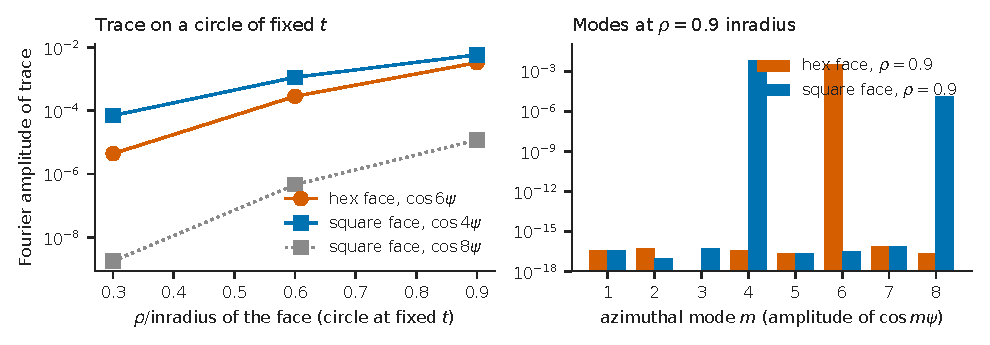
\includegraphics[width=\linewidth]{fig/fig_traces.pdf}
\caption{\tier{X} Fourier amplitudes of $h_{\rm bcc}$ on circles of fixed in-face radius (fixed $t$) on a hexagonal and a square face. Left: amplitude of the single nonzero mode against $\rho/$inradius. Right: all modes 1--8 at $\rho=0.9$ inradius; bars near $10^{-16}$ are round-off. Code-generated from \texttt{code/n3\_green\_obstruction.json}.}\label{fig:traces}
\end{figure}
This is what we measure (\cid{X-0004}; Figure~\ref{fig:traces}). On the hexagonal face the maximum minus the minimum of the trace is
$\BHexA$, $\BHexB$, $\BHexC$ at $\rho/{\rm inradius}=0.3,0.6,0.9$, its only Fourier content is $\cos6\psi$ (amplitude $\BHexSixC$ at $0.9$) and every other mode up to 8 is below $\BOffHex$.
On the square face the only modes are $\cos4\psi$ ($\BSqFourC$ at $0.9$) and $\cos8\psi$. The $6$-fold symmetry on the hexagonal face follows from
inversion through the face centre combined with the 3-fold axis. The planar proof has no analogue of these modes because a line carries no azimuth.
The face trace is representable by an in-face Chebyshev-type ansatz (\tier{C}; only modes up to 8 were measured); what remains for the hierarchical class is the interior of the hexagonal pyramid, which has only
$C_{3v}$ symmetry and cannot be $R$-invariant. Removing it needs data from the neighbouring faces, which leaves the piece-intrinsic class.

\subsection{Results and exact scope}\label{sec:scope-neg}
\begin{table}[t]
\centering\small
\begin{tabular}{@{}p{0.43\linewidth}ccc@{}}
\toprule
Trial class & forced slack $\ge$ (per particle) & / (fcc$-$bcc gap) & tier\\
\midrule
radial & \BSlackRadial & \BRatioRadial & X\\
axial (combined bound) & \BSlackAxial & \BRatioAxial & X\\
\quad of which hexagonal pyramids (pair average) / azimuthal only & $\BSlackHier$ / \BSlackAxHex & -- & X\\
\quad square pyramids (azimuthal) & \BSlackAxSq & -- & X\\
hierarchical, piece-intrinsic (hexagonal pyramids) & \BSlackHier & \BRatioHier & X\\
2D reference: radial, against the square$-$triangular gap & \BDRadTwoD & \BDRatioTwoD & X\\
2D reference: sector ansatz & $0$ (identity) & 0 & C\\
\bottomrule
\end{tabular}
\caption{Forced square term at the bcc torus (unit density, per-particle units). The fcc$-$bcc gap is \BGapFcc{} (hcp$-$bcc: \BGapHcp). Sobol quasi-Monte Carlo, replicate seeds 11 and 12 agree to about $10^{-7}$ for the axial and hierarchical rows (radial: $4\times10^{-6}$, within one standard error) (axial \BSeedAxA{} and \BSeedAxB; hierarchical \BSeedHierA{} and \BSeedHierB).}\label{tab:slack}
\end{table}
\begin{figure}[t]
\centering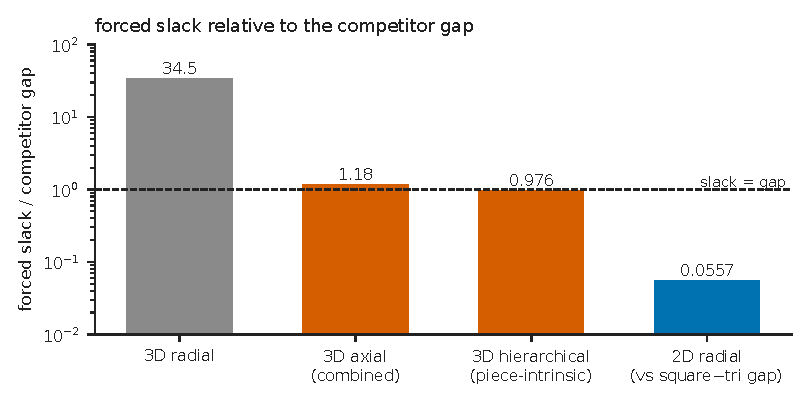
\includegraphics[width=0.72\linewidth]{fig/fig_slack.pdf}
\caption{\tier{X} Forced slack divided by the competitor gap, by trial class (log scale; the 3D classes are measured against the fcc$-$bcc gap, the 2D class against the square$-$triangular gap). Code-generated from \texttt{code/n3\_green\_obstruction.json}. The planar sector ansatz has slack zero by the manuscript identity and cannot be drawn on a log axis.}\label{fig:slack}
\end{figure}

\begin{proposition}[negative outcome, with scope; \cid{X-0006}, built on \cid{C-0011}, \cid{C-0012}, \cid{C-0013}, \cid{X-0004}, \cid{X-0005}]
For a certified constant $C$ obtained from a trial class that is radial, axial, or piece-intrinsic hierarchical in the sense above,
$C\le W_{\rm bcc}-\delta$ with $\delta\ge\BSlackRadial$, $\BSlackAxial$, $\BSlackHier$ respectively, \emph{provided the floating-point slack values are correct}.
In particular, no such class reproduces $W_{\rm bcc}$.
\end{proposition}
\textbf{What is and is not claimed.} The logic is the Pythagorean one of Lemmas~\ref{lem:slack}--\ref{lem:ceiling}, which is \tier{C}; its
evaluation at bcc is \tier{X}. The slack values are Monte Carlo estimates with standard errors (about $3\times10^{-7}$ for the hierarchical bound, i.e.
about \BNSigmaHier{} standard errors from zero; about \BNSigmaAx{} for the axial bound), not interval enclosures. The reported standard error is the iid formula applied to one scrambled Sobol sequence per seed, a heuristic and not a randomized-QMC confidence interval, and two replicates are not a confidence interval either; strict positivity does not depend on it, since the integrands are pointwise non-negative and bounded away from zero on open sets. The obstruction is
\emph{strict positivity}, not the size: a slack of $0.98$ times the gap is as fatal for exact calibration as $1.18$ times. The comparison with the fcc--bcc
gap is scale context: the best deficit is of the order of the distance to the nearest competitor, so the best certified constant from these classes lies below $W_{\rm bcc}$ by at least about the fcc--bcc gap; such a certificate could not exclude a hypothetical configuration whose energy is below $W_{\rm bcc}$ by less than that amount. The statement does \emph{not} apply to ansatz classes that are not invariant under the $60^\circ$ rotation, for example classes carrying neighbour data (Section~\ref{sec:count}).

\section{Numerics with controls (Tier X)}\label{sec:num}
All numbers come from \texttt{code/} (copied from the study's \texttt{numerics/}); the figures and the macros in \texttt{gen\_numbers.tex} are generated by \texttt{make\_all.py} from
the JSON files; the exceptions are the Muratov--Novaga margin (quoted from their eq.~(11)) and the 2D lattice energies $W_{\rm tri}=-4.1504128077$, $W_{\rm square}=-4.1171606$ (typed constants in the code, taken from the manuscript normalization as quoted in the earlier audit and not recomputed). The fcc--bcc gap is taken from the computed energies of \texttt{n1\_energies.py}, not from the hand-typed constant in the slack script. Energies are Ewald sums for the one-component plasma at unit density.

\textbf{Energies and controls} (\cid{X-0001}). bcc $\BEBcc$; fcc above bcc by \BGapFcc{} (relative \BRelGapFcc, consistent with Muratov--Novaga's $6.2\times10^{-5}$, \tier{C} \cid{C-0005}); hcp by \BGapHcp.
Our value $2\times$ the fcc gap, \BTwoGap, agrees with Muratov--Novaga's margin \BMNMargin{} in their normalization (energy twice ours; eq.~(11) of their paper).
Positive controls: independence of the Ewald splitting parameter to \BAlphaSpread; literature Madelung constants reproduced to \BMadDev{} (bcc, fcc, hcp) and \BMadDevSc{} (sc); the constants in \texttt{n1\_energies.py} are hard-coded, and the independent audit checked them against Table~III of Alves et al.~\cite{alves} (and Muratov--Novaga eq.~(5), Kozhberov arXiv:2411.03863), which agree to the printed digits. Negative control: dropping the background term makes the result depend on the splitting parameter (spread \BNegSpread).

\textbf{Green function checks} (\cid{X-0003}). The finite-difference Laplacian off the sites is \BLapFD{} against $4\pi=\BLapExp$; the analytic gradient agrees with central differences to \BGradDev.
The regular constant of $h_{\rm bcc}$ near the site, \BCReg, matches $2\times$ Madelung $=\BTwoMad$ (positive control); the degree-4 cubic-harmonic coefficient is $c_4=\BCFour$ (bcc), $\BCFourFcc$ (fcc), $\BCFourSc$ (sc), so the cubic-harmonic channel of the 3D tails is nonzero.

\textbf{Slack bounds} (\cid{X-0005}). Positive (null) control: replacing $h$ by the exactly radial Wigner--Seitz field gives \BWSAx, \BWSRad, \BWSHier{} for the axial, radial and hierarchical bounds, i.e.\ zero to round-off. This control alone does not test the rotation convention
of the pair-average bound (a radial field is invariant under every rotation). \emph{Independent-auditor result} (not run by the authors of the study; script \texttt{/tmp/b3audit/ctl.py} of the auditor, a scratch file not shipped here; numbers as reported in \texttt{AUDIT.md}; the paper's own \texttt{bounds\_for\_gradient} on $2^{16}$ scrambled Sobol points, seed 5, in one hexagonal pyramid): a non-radial field invariant under rotation about $\hat n$, $f=(n\!\cdot\!x)^3+\rho^4$, gives hierarchical bound $5.4\times10^{-35}$ and axial $3.9\times10^{-36}$ (full Dirichlet energy $1.28\times10^{-3}$); $\mathrm{Re}(u+iv)^6$ ($\cos6\psi$, $R$-invariant but not axial) gives hierarchical $3.0\times10^{-37}$ and axial $2.8\times10^{-7}$; $\mathrm{Re}(u+iv)^3$ ($\cos3\psi$, odd under $R$) gives hierarchical $1.29994\times10^{-4}$, equal to its full Dirichlet energy $1.29994\times10^{-4}$, as predicted since $(1-R)/2=1$ on that mode. So the convention in the code is correct (\tier{X}, auditor). The 2D reference (\texttt{two\_d\_reference}) is plain Monte Carlo with $4\times10^5$ points, reports no standard error, and its Monte Carlo hexagon area is $1.0011$. The bcc cell volume by Monte Carlo is within $2\times10^{-4}$ of 1 for both seeds. The earlier run archived as \texttt{n3\_run1\_pre\_signfix.json} contained an $r^2$ sign error in the cubic fit and in the control field and lacked the combined axial bound; its slack bounds agree with the final run, which is the one cited.

\textbf{Per-cell comparisons} (\cid{X-0002}; Table~\ref{tab:cells}, Figure~\ref{fig:energyG}).
\begin{table}[t]
\centering\small
\begin{tabular}{@{}lrrrrr@{}}
\toprule
Configuration & $N$ & $e-e_{\rm bcc}$ & mean faces & mean $\sum(6-n_F)$ & $G$\\
\midrule
\BTableConfigs
\bottomrule
\end{tabular}
\caption{Periodic Voronoi statistics and jellium energy above bcc (\tier{X}). The mean Euler weight is 12 for simple cells; fcc and hcp have non-simple cells (negative control, 24). $G$ is the dimensionless second moment of the cell.}\label{tab:cells}
\end{table}
\begin{figure}[t]
\centering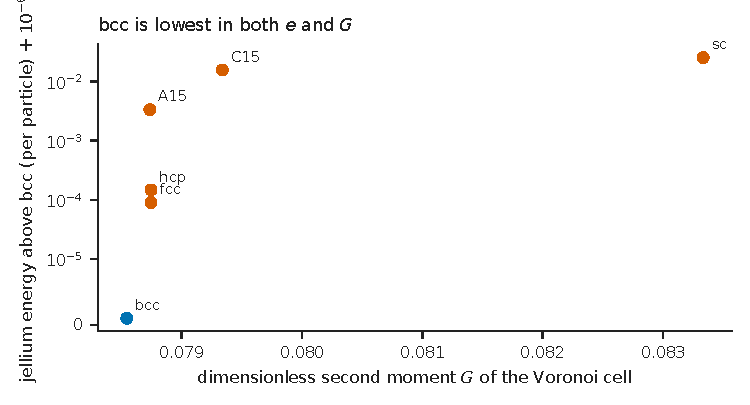
\includegraphics[width=0.72\linewidth]{fig/fig_energy_G.pdf}
\caption{\tier{X} Jellium energy above bcc against the second moment $G$ of the Voronoi cell for the six crystal structures (symmetric-log axis; bcc is shifted by $10^{-6}$ to be drawn; the fcc--bcc gap is $10^{-4}$ in $e$ and $2\times10^{-4}$ in $G$). Code-generated from \texttt{code/n1\_energies.json} and \texttt{code/n2\_voronoi.json}.}\label{fig:energyG}
\end{figure}
Four observations. (1) bcc is not extremal in the number of faces, so no per-cell count that is sharp at bcc can be a face count (hence the Euler weight of Section~\ref{sec:euler}).
(2) The Euler weight is $12$ on \BNEulerCfg{} of \BNCfgAll{} configurations; fcc and hcp give 24; one perturbed hcp run gave \BHcpArtifact, which is impossible for convex cells and which we attribute, without independent check, to a near-degenerate-vertex merge at the $10^{-7}$ tolerance. (The study note quoted 33 configurations; the result file holds \BNCfgAll, which is what we report.)
(3) The Weaire--Phelan cells (A15), which beat bcc for the Kelvin surface-area problem~\cite{ai}, lose to bcc in jellium energy by $3.4\times10^{-3}$ and in quantization by $1.9\times10^{-4}$ in $G$: the jellium question does not inherit Kelvin's counterexample.
(4) A per-cell functional that is sharp at bcc must nevertheless separate cells that differ by $6\times10^{-5}$ in relative energy.

\section{The count and the Euler identity}
\subsection{The incidence count transfers}\label{sec:euler}
\begin{proposition}[cell Euler identity; \tier{C}, \cid{C-0014}]
For a convex polyhedron with $f$ faces, $e$ edges, $v$ vertices, $v-e+f=2$. Each vertex has degree $\ge3$, so $3v\le2e$, hence $e\le3f-6$ and $\sum_Fn_F=2e\le6f-12$, i.e.\ $\sum_F(6-n_F)\ge12$, with equality iff the cell is simple. For a simple cell $\sum_F(6-n_F)=12$ exactly, whatever $f$ is.
\end{proposition}
(The rhombic dodecahedron of fcc has $f=12$, $e=24$, $\sum(6-n_F)=24$, consistent with the table.) With the sector weight $K(3\theta'_e/\pi-1)$ of the planar proof, a face with its foot inside sums to
$K(6-n_F)$ and a foot outside gives $-Kn_F\ge K(6-n_F)$ when $K\le0$; tiny faces near degenerate vertices force $K\le0$. The count therefore transfers
with $K\le0$ as in 2D (\tier{C} sketch, \cid{C-0015}, not carried out in detail), after one extra step. Unlike 2D, the Euler inequality $\sum_F(6-n_F)\ge12$ points in the unfavourable direction for $K\le0$ (non-simple cells such as those of fcc and hcp give $24K$). The transfer therefore uses an extra step: configurations with simple Voronoi cells are dense, and $W_N$ is continuous on separated configurations, so it suffices to prove the bound for simple tessellations, on which $\sum_F(6-n_F)=12$ exactly; the certificate domain must then include a margin below the separation distance (as the planar proof's $b=0.28209<d_*$ does) to cover nearby perturbations. \emph{This is not the failing step.}

\subsection{The calibration count is overdetermined}\label{sec:count}
Which additive invariants have a fixed total per simple cell? From $v=2f-4$ and $\sum n_F=6f-12$, $af+b\sum n_F+cv=(a+6b+2c)f-12b-4c$ is constant iff $a+6b+2c=0$ (\tier{C}, \cid{C-0017}),
so, besides volume ($\lambda$) and total solid angle ($\mu$), the only free count weight is the Euler one ($K$): three multipliers.

The truncated octahedron has $144$ flags and $O_h$ has order $48$: three flag orbits, hence three in-face sector types (square face with a hex--square edge; hexagonal face with a hex--square edge; hexagonal face with a hex--hex edge). Piece-intrinsic data see two types; neighbour data split the hexagonal type.
A per-piece affine bound that is tight at bcc imposes three stationarity conditions and one equality per type: about $8$ conditions (two types) or $12$ (three types) against $3$ multipliers, whereas in 2D one sector type gives $2+1=3$ conditions for $3$ multipliers
(\tier{C}, \cid{C-0018}). This is a \emph{counting heuristic}, not a theorem: hidden identities coming from the stationarity of $W$ at bcc are not excluded. It is the only argument against ansatz classes whose data are not invariant under the $60^\circ$ rotation of the hexagonal pyramids (in particular, classes that carry neighbour data, whatever their number of parameters), and it is a negative of Tier~C strength only.

\subsection{The cell-local relatives}\label{sec:cells}
The planar proof also leans on the hexagon being optimal for a scalar cell functional (the Fejes T\'oth/Gruber pattern). In 3D the corresponding cell-local problems are open or false:
Gersho's conjecture on quantizers is open for $d\ge3$ and bcc is known to be optimal among lattice quantizers~\cite{ai} (\tier{C} \cid{C-0003}); Kelvin's conjecture was refuted by Weaire--Phelan~\cite{ai}; the dodecahedral bound of Hales--McLaughlin~\cite{hm} is for a cell that is not a tiling cell, so a per-cell bound need not be sharp at the optimum (\tier{C} \cid{C-0006}, abstract only).
In our numerics $G$ is lowest at bcc among the tilings tried (Table~\ref{tab:cells}), so quantization does not refute bcc, but it is a different functional.

\section{A residual, non-sharp target and how it can fail}\label{sec:plan}
The ceiling of Lemma~\ref{lem:ceiling} suggests a weaker goal (\tier{C}, \cid{C-0020}): a computer-assisted lower bound $W\ge W_{\rm bcc}-\delta^*$ with $\delta^*$ as small as the class allows, using the 3D dual identity with the axial ansatz. For the axial class $\delta^*\ge\BSlackAxial$, against the Lieb--Narnhofer gap of $6.6\times10^{-3}$; the radial class alone has the ceiling $W_{\rm bcc}-\BSlackRadial\approx-1.4473$ (\tier{X}, \cid{X-0008}), which would improve on $-1.4508$ by $3.5\times10^{-3}$ \emph{if} attained; it is an upper limit for the radial class, and whether any radial certificate approaches it is untested (a certificate must hold at the worst configuration, so its constant could lie anywhere at or below $-1.4473$). These are ceilings of what the method could deliver, not bounds we have.

\textbf{First lemma.} The 3D torus pipeline G2+G3+G5+G6 on paper: separation $R=(3/4\pi)^{1/3}$ (the identities $\phi(R)=\phi'(R)=0$ and $-\Delta\phi=4\pi(\delta-1_{B_R})$ for $\phi=1/|x|-3/(2R)+|x|^2/(2R^3)$ are checked by hand, \tier{C} \cid{C-0016}), the axial dual identity on flat tori of volume $N$, and the in-face signed-sector reduction G7 to the primitive $\Gamma_{d,s}(x)$.

\textbf{Falsification test (run first; not yet run).}
\begin{enumerate}
\item Optimize the axial radial data $B$, $D_k$ to maximize the calibrated constant $12K+\lambda+4\pi\mu$.
\item Sample random in-face sectors ($d\ge0.31$; $s$, $x$ arbitrary) and check that the piece inequality holds.
\item Kill the plan if the best feasible constant does not beat the Lieb--Narnhofer constant $-1.4508$ (or an actually certified radial constant), i.e.\ if the angular modes add nothing. (The radial ceiling $\approx-1.4473$ is not the right yardstick: it is an upper limit, not an achievable radial certificate.)
\end{enumerate}
A secondary target is $\delta^*<6.6\times10^{-4}$, ten times better than Lieb--Narnhofer. Against the preregistered priors (credible plan $0.15$, proof $0.02$), the outcome is ``no credible plan for a proof of bcc optimality with this architecture, a credible plan only for a weaker bound'', which is below the prior for the optimality question.

\section{Certificate-size estimates (Tier C, explicit assumptions)}\label{sec:cert}
Planar record, as quoted in our note from the manuscript's verification data: an outer mesh of about $2184\times3611\approx\BNodesTwoD$ nodes, a Hessian mesh of about $2.4\times10^6$ cells, about $4.2\times10^5$ global-derivative rectangles, 39 modes, worst margin $1.2\times10^{-5}$, $72.6$\,s on 32 threads ($\approx2.3\times10^3$ core-seconds).
Assumptions: (a) best case, exact axial pieces with a primitive in 3 variables; (b) margins scale with the relative gap of the nearest competitor, $8.0\times10^{-3}$ in 2D against $6.2\times10^{-5}$ in 3D, a factor of \BMarginRatio; (c) interpolation error $\propto h^2$, so a mesh \BRefine{} times finer per dimension; (d) the same cost per node (about \BEpsPerNode{} core-seconds, counting all three planar meshes), ignoring the larger cubic-harmonic channel count.
Under (a)--(d) a uniform mesh needs $(2808\times\BRefine)^3\approx\BNodesThreeD$ nodes, of the order of \BCoreYears{} core-years; an exact ansatz with five parameters would need about \BNodesFiveD{} nodes, infeasible uniformly. Adaptive boxes as in Muratov--Novaga (46\,414 boxes in five dimensions at the same relative gap, \tier{L} \cid{L-0002}) suggest $10^5$--$10^8$ boxes if a sharp piece inequality existed (\tier{C}, \cid{C-0021}).
So the size of the certificate is \emph{not} the binding constraint; the existence of a sharp piece inequality is.

\section{Limitations}
\begin{itemize}
\item \textbf{Two scopes.} The negative is a strict-positivity statement for the radial, axial and piece-intrinsic hierarchical classes of Section~\ref{sec:obstruction}, resting on a \tier{C} lemma and \tier{X} evaluations; for richer classes it rests on the \tier{C} counting heuristic only.
\item \textbf{Floating point.} The slack bounds are quasi-Monte Carlo (about $2^{19}$ points per cell, two seeds); there are no enclosures, and the pair-average rotation convention is covered only by the independent auditor's rotation control (Section~\ref{sec:num}), not by the study's own null control.
\item \textbf{Lower bounds, not values.} The classes give lower bounds on the square term; the true best slack of a class may be larger. The square pyramids are not used in the hierarchical bound, and a group average over the cyclic group $C_6$ (instead of the pair average) would give larger bounds; they were not computed. (We do not claim reflection invariance of the piece-intrinsic class, since oriented in-face data need not be mirror-symmetric, so the dihedral group is not used.)
\item \textbf{Not machine-checked.} Nothing here is formalized. The dual identity omits the renormalization bookkeeping at the sites (inherited from the planar proof); the cutoff-dependence caveat of G1 for $d\ge3$ is unresolved.
\item \textbf{Conditional on the planar proof being right.} We take the AI-generated planar proof as given (audit: no gap found in Sections~2--5), and we did not re-read it ourselves; the independent audit re-read its calibration section and found our description of G5--G9 accurate.
\item \textbf{Literature.} Quotations from Blanc--Lewin, Lewin, Aydın--Iacobelli, Rougerie--Serfaty Remark~B.2 and Muratov--Novaga Section~7 are verbatim but are remarks, hence filed at C. The Lieb--Narnhofer paper, Weaire--Phelan, Gersho, Barnes--Sloane, Choksi--Lu and the cited 2026 lattice result are second-hand (as reported in the surveys above). Hales--McLaughlin: abstract and first page only. Graf--Schenker, mentioned in the study note, was never read and is not cited.
\item \textbf{No audit.} No human audit of this preprint has been done. One independent AI audit (\texttt{AUDIT.md}, a separate Claude agent instance, verdict accept with corrections) has been done and its corrections are applied in this version; an AI audit is not a substitute for human review.
\end{itemize}

\section{Reproducibility}
From the paper directory (\texttt{papers/p2\_3d\_feasibility/}), with the project interpreter \texttt{.venv/bin/python}:
\begin{verbatim}
python -I code/n1_energies.py           # energies, controls
python -I code/n3b_cubic.py             # cubic fit
python -I code/n2_voronoi.py            # Voronoi statistics
python -I code/n3_green_obstruction.py  # slack bounds, ~45 min
python -I make_all.py                   # figures, macros
python -I ledger/run_citations.py       # Tier-L gate
python -I ledger/build_ledger.py && python -I ledger/run_gate.py
\end{verbatim}
Each script writes its JSON next to itself. At paper stage we re-ran \texttt{n1\_energies.py} and \texttt{n3b\_cubic.py} under \texttt{python -I} and they reproduced the stored JSON byte for byte; \texttt{n2\_voronoi.py} and \texttt{n3\_green\_obstruction.py} were \emph{not} re-run (the cited results are the study's own runs). Compute for the study: cores 6--7, 2 threads, about 45 minutes in total. The study was committed in the AutoevolveAI repository at the commit recorded in
\texttt{publication\_meta.json}. Source texts of the Tier-L rows are not redistributed; \texttt{ledger/sources/MANIFEST.md} lists their hashes and the re-fetch recipe.
The Elenchus gate (\texttt{tools/ledger.py}) is run with \texttt{--evidence-dir ledger/evidence}; its verbatim output and exit code are in \texttt{ledger/gate\_output.txt}. A clean gate is bookkeeping only; it licenses nothing.
Where this paper overrides statements of the internal study note shipped in \texttt{data/} (the rigour claim, the meaning of tier ``A'', the number of configurations, the $W_{\rm fcc}$ phrases, the ``D6'' labels), \texttt{data/SUPERSEDED\_STATEMENTS.md} lists the overridden statements; the paper's text governs.

\begin{thebibliography}{99}\small
\bibitem{oai} openai/math release: ``Triangular minimality for planar Coulomb renormalized energy'' (2026-09-23). AI-generated, not peer reviewed. Not re-read at paper stage.
\bibitem{audit} X.~Callens, ``Sandier--Serfaty conjecture: reproduction of a finite certificate, audit of the reduction, Lean statement'', Zenodo, doi:10.5281/zenodo.23653827 (2026). AI-produced, not peer reviewed.
\bibitem{mn} C.~B.~Muratov, M.~Novaga, arXiv:2610.29732v1. Read (full text): Theorem~1 (p.~4), Proposition~6 (p.~13), p.~3 and Section~7 (p.~14).
\bibitem{lw} S.~Luo, J.~Wei, arXiv:2610.31456v1. Read: Theorem~1.1.
\bibitem{rs} N.~Rougerie, S.~Serfaty, ``Higher dimensional Coulomb gases and renormalized energy functionals'', arXiv:1307.2805v5 (Commun.\ Pure Appl.\ Math.\ 69 (2016) 519). Read: Theorem~1 (p.~12), Remark~B.2 (p.~67).
\bibitem{bl} X.~Blanc, M.~Lewin, ``The crystallization conjecture: a review'', arXiv:1504.01153v2 (EMS Surv.\ Math.\ Sci.\ 2 (2015) 255). Read: Section~2.6 (p.~19).
\bibitem{lewin} M.~Lewin, arXiv:2202.09240v2 (J.\ Math.\ Phys.\ 63 (2022) 061101). Read: Remark~19 (p.~22). Survey; the original Lieb--Narnhofer paper (J.\ Stat.\ Phys.\ 12 (1975) 291) was \emph{not} read.
\bibitem{ai} A.~D.~Ayd{\i}n, M.~Iacobelli, arXiv:2610.28547v1. Read: abstract, pp.~4--6. Weaire--Phelan, Gersho, Barnes--Sloane, Choksi--Lu are taken from this paper (second-hand).
\bibitem{alves} E.~Alves, P.~Bendazzoli, S.~Evangelisti, J.~A.~Berger, arXiv:2103.01622. Table~III (Madelung constants $\eta_0$ of bcc, fcc, hcp, sc), used by the independent audit to check the constants in \texttt{n1\_energies.py}.
\bibitem{hm} T.~C.~Hales, S.~McLaughlin, ``The dodecahedral conjecture'', arXiv:math/9811079v3. \emph{Abstract and first page only.}
\end{thebibliography}
\end{document}
